\scanpage{90}

\[
\text{(24)}\qquad |\lambda_1|\mathord{-}|\lambda_n|=\rho_1\mathord{-}\rho_n
\]

\deleted{En effet, le \deleted{\unsure{produit}}\inserted{carré du premier} mb est égal à \deleted{$|\lambda_1\unsure{\rho|q}$} $|\lambda_1\mathord{\cdot}\,\mathord{-}\lambda_n|^2=|\det u|^2=(\overline{\det u},\unsure{\overset{\deleted{\mathrm{conj}}}{\det u}|\overline{\det u}})=(\det u^*)\det u\deleted{{}^{\unsure{*}}}=\det u^*u=\rho_1^2\mathord{-}\,\mathord{-}\rho_n^2$, où $\rho_1\mathord{-}\rho_n$ sont les valeurs propres de $(u^*u)^{1/2}$, d'où (23).}
\textcolor{red}{\uline{\textcolor{black}{Il \deleted{\unsure{que}} \inserted{\deleted{\unsure{d'où}}} s'ensuit, \unsure{ainsi|alors},}}}

\reversemarginpar
\margin{On a \deleted{\unsure{d'autre|d'une part} $\unsure{\lambda_1}\mathord{-}\lambda_n=\det\inserted{\deleted{\unsure{u}}}$}
\begingroup\setbox0=\hbox{$\text{(25)}\quad\lambda_1(u)\mathord{-}\lambda_n(u)=\det u$}\dimen0=\wd0\advance\dimen0 by6pt\dimen2=\ht0\advance\dimen2 by3pt\dimen4=\dp0\advance\dimen4 by3pt\dimen6=\dimen4\advance\dimen6 by-2pt\leavevmode\hspace{3pt}\rlap{\begin{tikzpicture}[overlay,baseline=0pt]\draw[line width=.45pt] (-3pt,\the\dimen2)--(-3pt,-\the\dimen4)--(\the\wd0,-\the\dimen4);\draw[line width=.45pt] (\the\dimen0,-\the\dimen6)--(\the\dimen0,\the\dimen2);\end{tikzpicture}}\box0\hspace{6pt}\endgroup
\deleted{et de} d'autre part $(\rho_1(u)\mathord{-}\rho_n(u))^2=\rho_1(u^*u)\mathord{\cdot}\,\mathord{-}\rho_n(u^*u)=\det(u^*u)=\det u^*\,\det u=\overline{\det u}\det u=|\det u|^2$, d'où
\begingroup\setbox0=\hbox{$\deleted{\unsure{(25)|(24)}}\ \text{\textcircled{26}}\quad\rho_1(u)\mathord{-}\rho_n(u)=\det|u|$}\dimen0=\wd0\advance\dimen0 by3pt\dimen2=\ht0\advance\dimen2 by3pt\dimen4=\dp0\advance\dimen4 by3pt\dimen6=\wd0\divide\dimen6 by10\dimen8=\wd0\advance\dimen8 by-\dimen6\dimen6=\dimen4\advance\dimen6 by-2pt\leavevmode\hspace{3pt}\rlap{\begin{tikzpicture}[overlay,baseline=0pt]\draw[line width=.45pt] (0pt,\the\dimen2)--(\the\dimen0,\the\dimen2);\draw[line width=.45pt] (-3pt,\the\dimen2)--(-3pt,-\the\dimen4)--(\the\dimen0,-\the\dimen4);\draw[line width=.45pt] (\the\dimen8,-\the\dimen4) to[out=70,in=180] (\the\wd0,-\the\dimen6);\end{tikzpicture}}\box0\hspace{3pt}\endgroup
En comparant (25) et (26), \unsure{tr.|t.} $\Rightarrow$ (24)}
\normalmarginpar

quand $u$ est inversible, \deleted{que} donc \deleted{$|\lambda_1\mathord{-}\lambda_n|$ \unsure{et}} les $\lambda_i$ et les $\rho_i$ non nuls \deleted{\unsure{que ce sont}}, que les conditions du \deleted{corollaire 1 du lemme fondamental 2 sont vérifiées, dans l'hypothèse b)} \inserted{\unsure{th.|Pr.} 1, 2\uuline{°}, hypo. b sont vérifiées.} Si on suppose que $f$ est de plus \textcolor{red}{\uline{\textcolor{black}{définie}}} et continue pour $r_i\geq0$, comme on aura (23) pour \deleted{tout} $u$ inversible et que les deux mbs sont des fonctions continues de $u$ comme on vérifie aussitôt, il s'ensuit que l'inégalité sera vérifiée pour \deleted{tout} $u$. -- Le

\deleted{\uline{Corollaire 5}} résulte p. ex du corollaire 4 que si $u$ est inversible, les formules (21) sont vérifiées $=$ si $p$ n'est pas positif. Notons que \deleted{sous les conditions du corollaire 3, on tire de \unsure{(24)|(26)} et des inégalités $|\lambda_1\mathord{-}\lambda_k|\leq\rho_1\mathord{-}\rho_k$, \unsure{les relations analogues}}

\reversemarginpar
\margin{\deleted{\unsure{(25)|(24)|(27)} $|\lambda_k\mathord{-}\lambda_n|\leq\rho_{\unsure{k|n}}\mathord{-}\rho_n$ $(1\leq k\leq n)$, \unsure{ce qui} \illegible{2} pour $\unsure{\rho_k}\mathord{-}\unsure{\rho_n}$, \illegible{3} \unsure{la} \illegible{2}} \textcolor{red}{\textcircled{?}}}
\margin{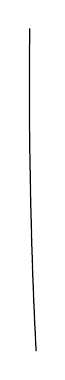
\begin{tikzpicture}[x=1cm,y=1cm]\draw[line width=.45pt] (0,0) .. controls (-.02,-1.05) and (.01,-2.85) .. (.08,-4.1);\end{tikzpicture}}
\normalmarginpar

\uline{Corollaire 5} Soit $u$ un opérateur dans un espace de Hilbert $E$, soit $N$ une norme de Schatten sur $R^{\deleted{I}\inserted{k}}$, \deleted{où $I=\deleted{\dim}(1,\unsure{\mathord{-}}n)$ \unsure{si} $\dim E=n$, et $I=$ ensemble des entiers si} \inserted{où $k\leq\dim E$.} \inserted{Alors, on a}

\[
\text{(27)}\qquad N(|\lambda_1|,\mathord{-}\,\mathord{-}|\lambda_k|)\leq N(\rho_1,\mathord{-}\,\mathord{-}\rho_k)
\]

\deleted{D'où, $\unsure{N(}\unsure{\leq|\xi|k|\lambda_i}$} Par suite, si la dimension de $E$ est infinie et si $N$ est une norme de Schatten sur \deleted{\unsure{tout|de}} l'espace $R^{(\underline N)}$, \deleted{\unsure{lorsque} $\underline N$ \unsure{désigne}} \inserted{on a}

\[
\text{\unsure{(28)|(26)}}\qquad N((|\lambda_i|))\leq N((\rho_i))
\]

Dans cet énoncé, $\underline N$ désigne l'ensemble des entiers, donc $R^{(\underline N)}$ l'espace des suites de \unsure{nbs réels|nbs entrs} \deleted{\unsure{qui sont}} dont seul un nb fini de termes sont non nuls. Une norme sur $R^{(\underline N)}$ est dite une norme de Schatten, si elle induit une norme de Schatten sur \deleted{tout} un, espace $R^n$ (plongé de façon naturelle dans $R^{(\underline N)}$).

\reversemarginpar
\margin{91}
\normalmarginpar
